\section{Theorie}

\subsection{Mikrowellen und Elektromagnetische Wellen }
Mikrowellen beschreiben elektromagnetische Wellen, die sich in einem vorher definierten Frequenzspektrum von 1 bis 300 $\si{\giga\hertz}$ befinden. 
Sie sind, im vergleich zu anderen alltäglichen Wellen, eher dem langwelligen Bereich zuzuordnen, weit jenseits dem für uns sichtbaren Lichts.
Elektromagnetische Wellen lassen sich hinreichend durch die Maxwell Glecihungen beschreiben, ohne jedoch dabei die Teilchen Eigenschaften der Korpuskeltheorie zu berücksichtigen. Im Folgenene Versuch wird sich außschließlich auf die Welleneigenschaften bezogen.
Charakteristisch für all diese Wellen ist die im Vakuum definierte Geschwindigkeit sich fortzubewegen, besser bekannt als Lichtgeschwindigkeit. Dort propagiert sie außschließlich als Transversalwelle.
Mit dieser Geschwindigkeit $c$, oder im Falle eines Mediums der entsprechend reduzierten, lässt sich nun die Wellenlänge mithilfe der Frequenz $\nu$ bestimmen.
\begin{equation}
\lambda = c/{\nu}
\end{equation}
Das Magnetische Feld verhält sich analog zum elktrischen, steht aber zu jedem Zeitpunkt senkrecht auf seiner elktrischen Komponente. \\  Große Anwendug 
finden diese \enquote{Mikrowellen} unter anderem in der Funk - und Radartechnik. Zum Beispiel werden so durch abweichende Brechungsindexe und wechselnden Impedanzen,  Inforationen durch reflektierte Wellen gewonnen. 
Eine weitere Anwendung ist der Mikrowellenherd, der mit einer Charakteristischen Frequenz von $\SI{2.455}{\giga\hertz}$ die Dipole von Wassermoleküle passend ausrichtet, anregt und so Wärme erzeugt.

\subsection{Reflexklystron}

Das Reflexklystron ist ein Gerät um hochfrequentige Wellen entweder zu verstärken oder selbstständig anzuregen. Grundlage dazu sind zwei angeschlossene Spannungen, 
die zum einem die Resonatorkammer und zum anderen den wortgebenen Reflektor elektrisch laden. Zudem wird eine Glühkathode verwendet, die aus möglichen Metallen, 
gegen eine Austrittsarbeit, freie Elektronen löst und in Richtung des Reflektors beschleunigt. Wolfram bietet sich hierfür aufgrund der sehr hohen Schmelztemperatur sehr gut an.
Diese nun beschleuigten Elektroden finden ihren Weg zum Reflektor durch die Resonatorkammer und werden anschließend in diese Kammer zurückgelenkt. Die anfangs anegelegte Spannung treibt 
die Elektronen im Resonator folglich schwingend in die Richtung, die der negativen Spannungskomponente entgegengesetzt ist. Durch diese frequente Ausrichtung des Elektrischen Felds werden die emittierten Elektronen entweder weiter beschleunigt oder 
verlangsamt, was zu einer frequenzabhängigen Modulation der Geschwindigkeit führt. Während die Beschleunigung von Elektronen dem Resonator Energie kostet gewinnt er diese zurück, wenn Elektronen gebremst werden. 
Eine für den Resonator optimnale Laufzeit für Energiegewinnung ist 
\begin{equation}
    \left(n+ \frac{3}{4} \right) \cdot T  \quad \quad n \in \mathbb{N}_0.
\end{equation}
Die so entstehende Schwingung wird anschließend durch einen Hohlwellenleiter ausgekoppelt und weiter transportiert.
\begin{figure}
    \centering
    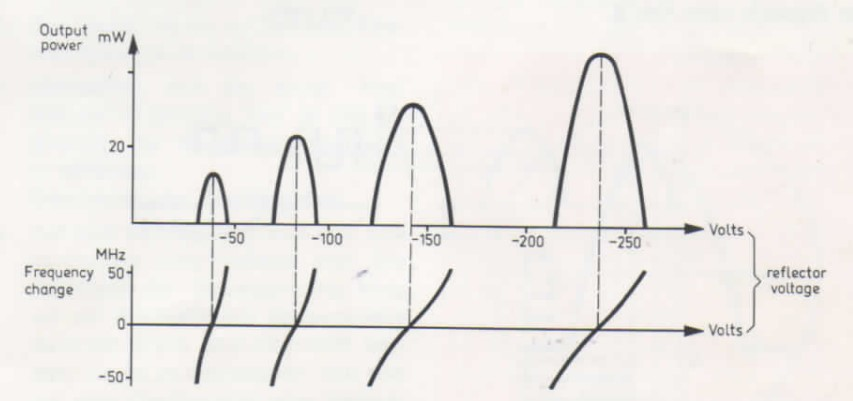
\includegraphics[width=0.8\textwidth]{bilder/dia.jpg}
    \caption{In Diesem Diagram ist die abgegriffene Leistug der Wellenmoden aus einem Reflexklystron, abhängig von der angelegten Reflektorspannung dargestellt.
    Die entsprechende Frequenz ist darunter mit gleicher Abszisse dargestellt. Deutlich erkennbar sind hier die einzelenen Moden die durch die Modulation entstehen.} 
    \label{fig:ref}
\end{figure}
\begin{figure}
    \centering
    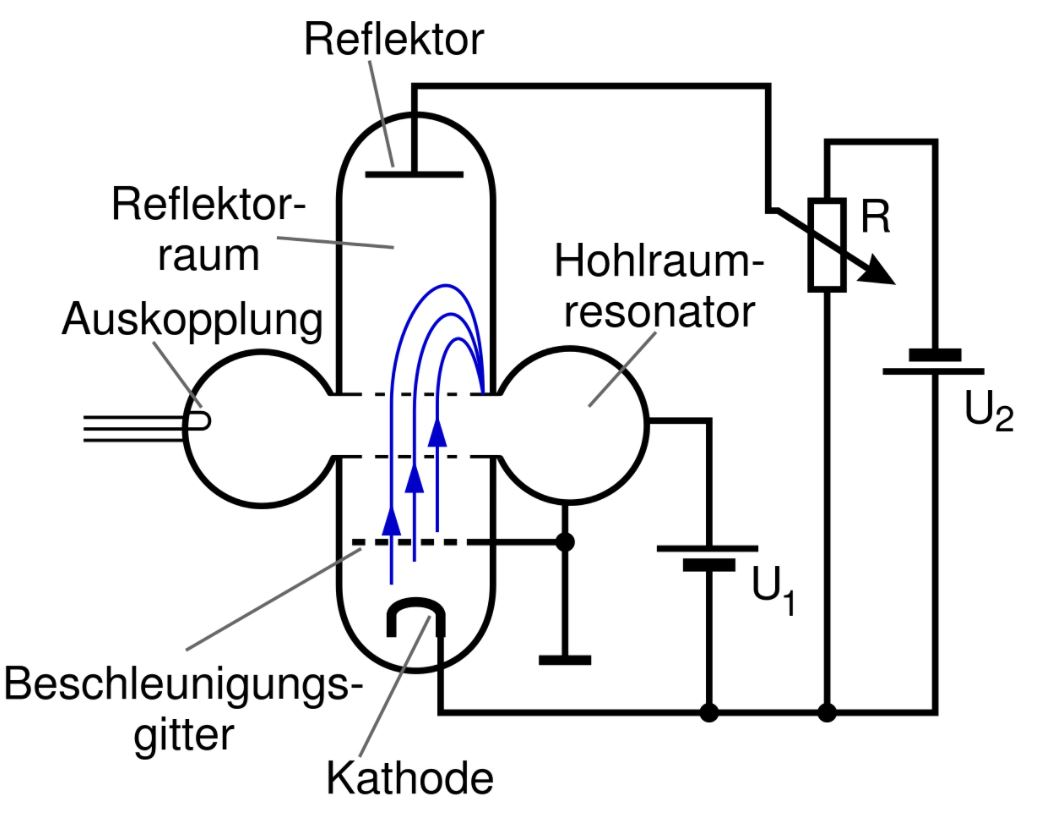
\includegraphics[width=0.6\textwidth]{bilder/theo.JPG}
    \caption{Schematischer Aufbau eines Reflexklystrons. Deutlich zu erkennen sind die blauen Pfeile, die verschiedene Elektronen abhängig von der angelegten Spannung darstellen. 
    Diese Sammlung an Elketronen nennt sich \enquote{Bunching}.} 
    \label{fig:ref}
\end{figure}
Durch Änderungen am internen Aufbau des Klystron lassen sich die Moden unteranderem durch Spannungsunterschiede verschieben. 
\begin{equation}
    P_{\text{Output}} (\si{\volt}) \sim P_{\text{Output}} (\si{\volt} + \tau)
\end{equation}
Die Variabel $\tau$ ist hier so gewählt, dass $\si{\volt} + \tau$ wieder die vorher von $\si{\volt}$ getroffene Mode beschreibt.
Analog lässt sich die Frequenz durch den mechanischen Aufbau ändern. Eine größere Resonatorkammer würder den Elektronen 
mehr Laufzeit bieten und so das \enquote{Bunching} verlangsamen.

